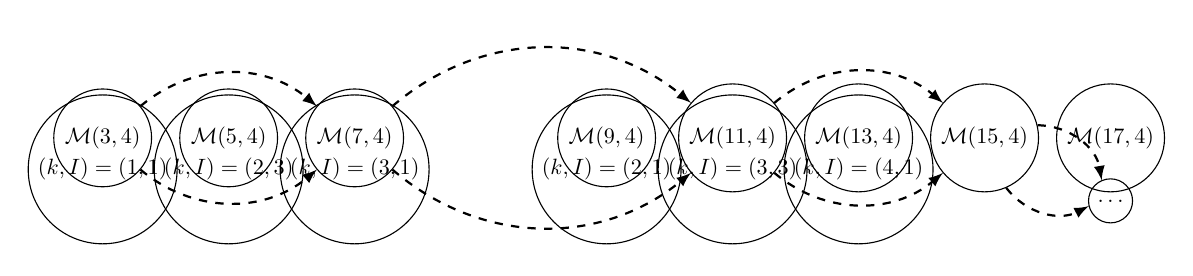
\begin{tikzpicture}[scale=0.8]
\tikzset{every node/.style={transform shape}}

%Nodes
\node[circle,draw=black] (A) at (-2,-3) {$\mathcal{M}(3,4)$};
\node[circle,draw=black] (B) at (0,-3) {$\mathcal{M}(5,4)$};
\node[circle,draw=black] (C) at (2,-3) {$\mathcal{M}(7,4)$};
\node[circle,draw=black] (D) at (6,-3) {$\mathcal{M}(9,4)$};
\node[circle,draw=black] (E) at (8,-3) {$\mathcal{M}(11,4)$};
\node[circle,draw=black] (F) at (10,-3) {$\mathcal{M}(13,4)$};
\node[circle,draw=black] (G) at (12,-3) {$\mathcal{M}(15,4)$};
\node[circle,draw=black] (H) at (14,-3) {$\mathcal{M}(17,4)$};

\node[circle,draw=black] (I) at (14,-4) {$\ldots$};


%Labels
\node[circle,draw=black] (J) at (-2,-3.5) {$(k,I)=(1,1)$};
\node[circle,draw=black] (K) at (0,-3.5) {$(k,I)=(2,3)$};
\node[circle,draw=black] (L) at (2,-3.5) {$(k,I)=(3,1)$};

\node[circle,draw=black] (M) at (6,-3.5) {$(k,I)=(2,1)$};
\node[circle,draw=black] (N) at (8,-3.5) {$(k,I)=(3,3)$};
\node[circle,draw=black] (O) at (10,-3.5) {$(k,I)=(4,1)$};

%Dashed Lines
\draw [dashed,->,>=latex,line width=0.8pt] (A) to[bend right=40] (C);
\draw [dashed,->,>=latex,line width=0.8pt] (C) to[bend right=40] (E);
\draw [dashed,->,>=latex,line width=0.8pt] (E) to[bend right=40] (G);
\draw [dashed,->,>=latex,line width=0.8pt] (G) to[bend right=40] (I);
\draw [dashed,->,>=latex,line width=0.8pt] (A) to[bend left=40] (C);
\draw [dashed,->,>=latex,line width=0.8pt] (C) to[bend left=40] (E);
\draw [dashed,->,>=latex,line width=0.8pt] (E) to[bend left=40] (G);
\draw [dashed,->,>=latex,line width=0.8pt] (G) to[bend left=40] (I);


\end{tikzpicture}